\documentclass{article}
\usepackage{setspace}
\usepackage[utf8]{inputenc}
\usepackage{natbib}
\usepackage{url}
\usepackage{indentfirst} 
\usepackage{hyperref}
\usepackage{xcolor}
\usepackage{float}

\usepackage{booktabs}
\usepackage{longtable}
\usepackage{array}
\usepackage{multirow}
\usepackage{wrapfig}
\usepackage{float}
\usepackage{colortbl}
\usepackage{pdflscape}
\usepackage{tabu}
\usepackage{threeparttable}
\usepackage{threeparttablex}
\usepackage[normalem]{ulem}
\usepackage[utf8]{inputenc}
\usepackage{makecell}
\usepackage{xcolor}

\usepackage{graphicx}
\graphicspath{ {figures/} }

\title{Constructing Optimal MLB Teams with Linear Programming}
\author{Nathan Schor}
\date{August 28, 2022}

\doublespacing
\begin{document}

\maketitle
\begin{singlespace}
\tableofcontents
\end{singlespace}

\section{Introduction}

\section{Literature Review}

\section{Methodology/Data}

%\begin{table}
%\caption{Number of Players who are on both the Optimal and Actual Teams}
%\label{tab:optimal_and_actual}
\begin{table}

\caption{For each team, the number of players selected for their optimal team who are also on their actual team}
\centering
\begin{tabular}[t]{|>{}l|>{\centering\arraybackslash}p{10em}|}
\hline
Team & Number of Players\\
\hline
\cellcolor{gray!6}{LAD} & \cellcolor{gray!6}{3}\\
\hline
WSN & 3\\
\hline
\cellcolor{gray!6}{MIL} & \cellcolor{gray!6}{2}\\
\hline
SFG & 2\\
\hline
\cellcolor{gray!6}{TBR} & \cellcolor{gray!6}{2}\\
\hline
ATL & 1\\
\hline
\cellcolor{gray!6}{BOS} & \cellcolor{gray!6}{1}\\
\hline
CHC & 1\\
\hline
\cellcolor{gray!6}{CIN} & \cellcolor{gray!6}{1}\\
\hline
COL & 1\\
\hline
\cellcolor{gray!6}{HOU} & \cellcolor{gray!6}{1}\\
\hline
LAA & 1\\
\hline
\cellcolor{gray!6}{MIN} & \cellcolor{gray!6}{1}\\
\hline
NYY & 1\\
\hline
\cellcolor{gray!6}{OAK} & \cellcolor{gray!6}{1}\\
\hline
PHI & 1\\
\hline
\cellcolor{gray!6}{PIT} & \cellcolor{gray!6}{1}\\
\hline
SDP & 1\\
\hline
\cellcolor{gray!6}{TOR} & \cellcolor{gray!6}{1}\\
\hline
CHW & 0\\
\hline
\cellcolor{gray!6}{NYM} & \cellcolor{gray!6}{0}\\
\hline
KCR & 0\\
\hline
\cellcolor{gray!6}{STL} & \cellcolor{gray!6}{0}\\
\hline
CLE & 0\\
\hline
\cellcolor{gray!6}{MIA} & \cellcolor{gray!6}{0}\\
\hline
BAL & 0\\
\hline
\cellcolor{gray!6}{ARI} & \cellcolor{gray!6}{0}\\
\hline
SEA & 0\\
\hline
\cellcolor{gray!6}{TEX} & \cellcolor{gray!6}{0}\\
\hline
DET & 0\\
\hline
\end{tabular}
\end{table}

%\end{table}

\begin{figure}[h]
\caption{Boxplot of Salary (for Players with Salary $> 0$) by Position}
\label{fig:salary_position_boxplot}
\centering
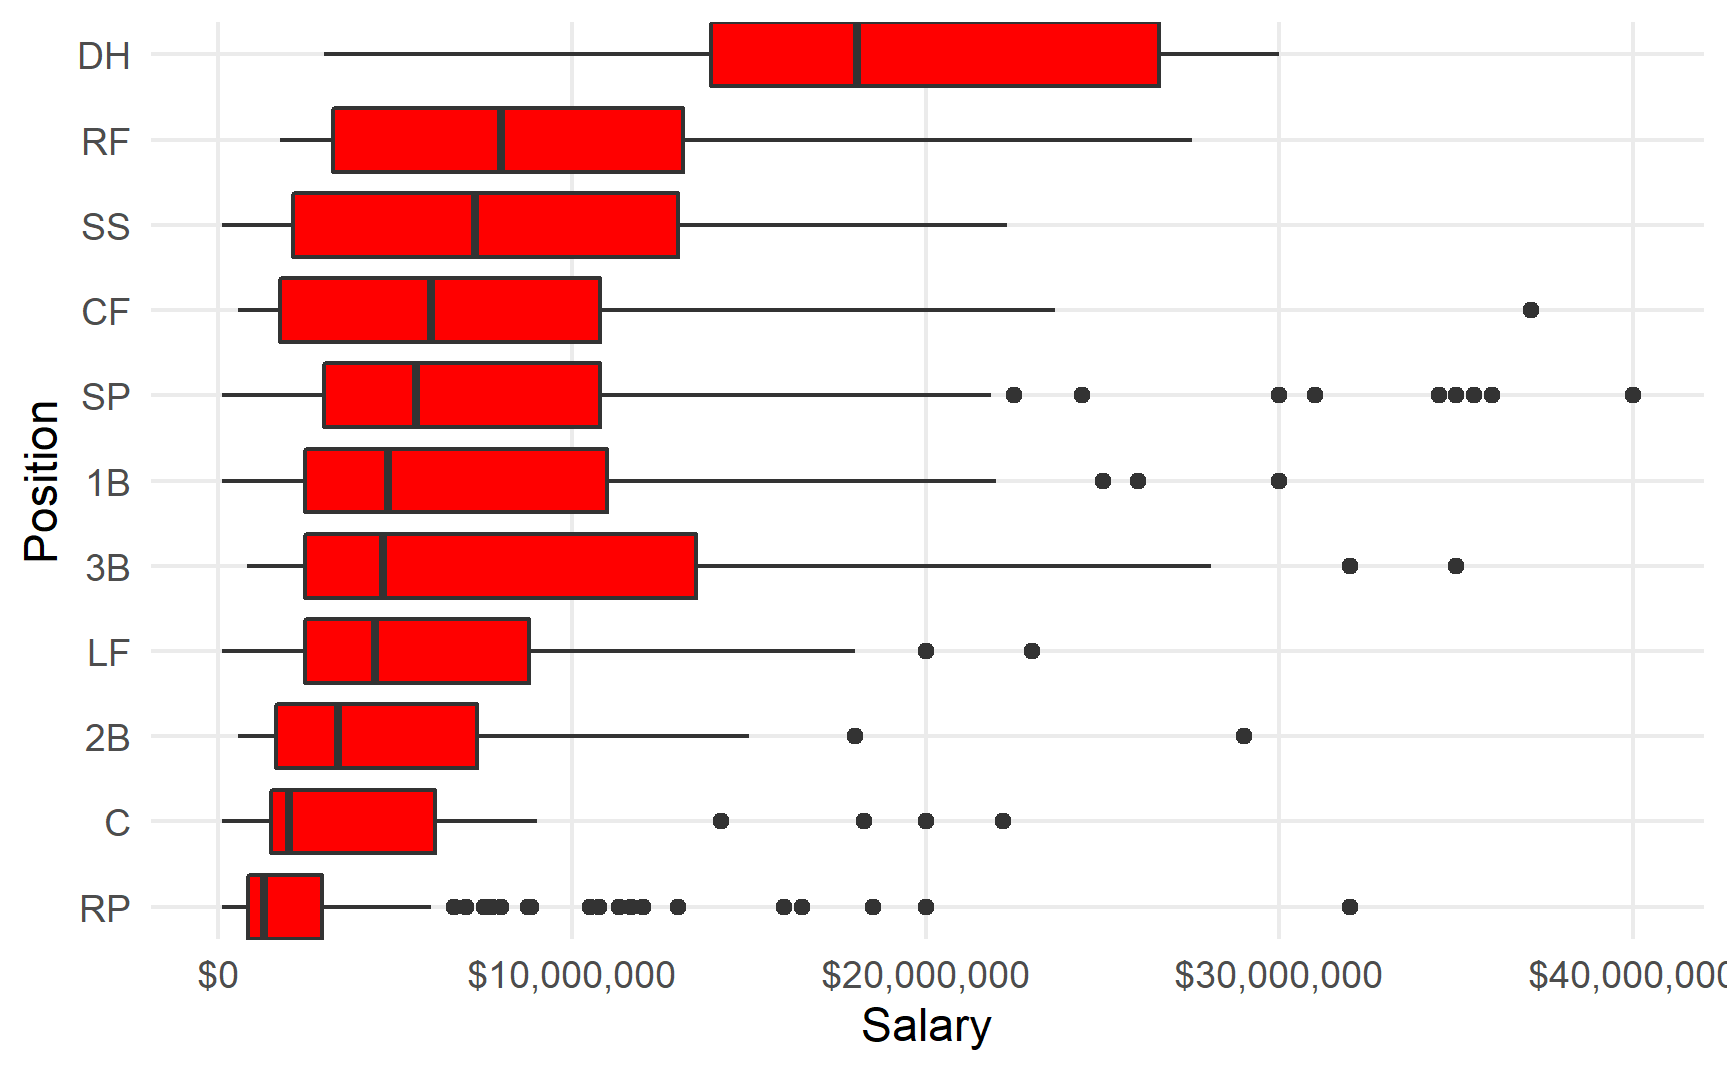
\includegraphics[width=0.7\paperwidth, scale=1.25]{salary_position_boxplots.png}
\end{figure}

\begin{figure}[h]
\caption{Boxplot of JEFFBAGWELL by Position}
\label{fig:salary_war_boxplot}
\centering
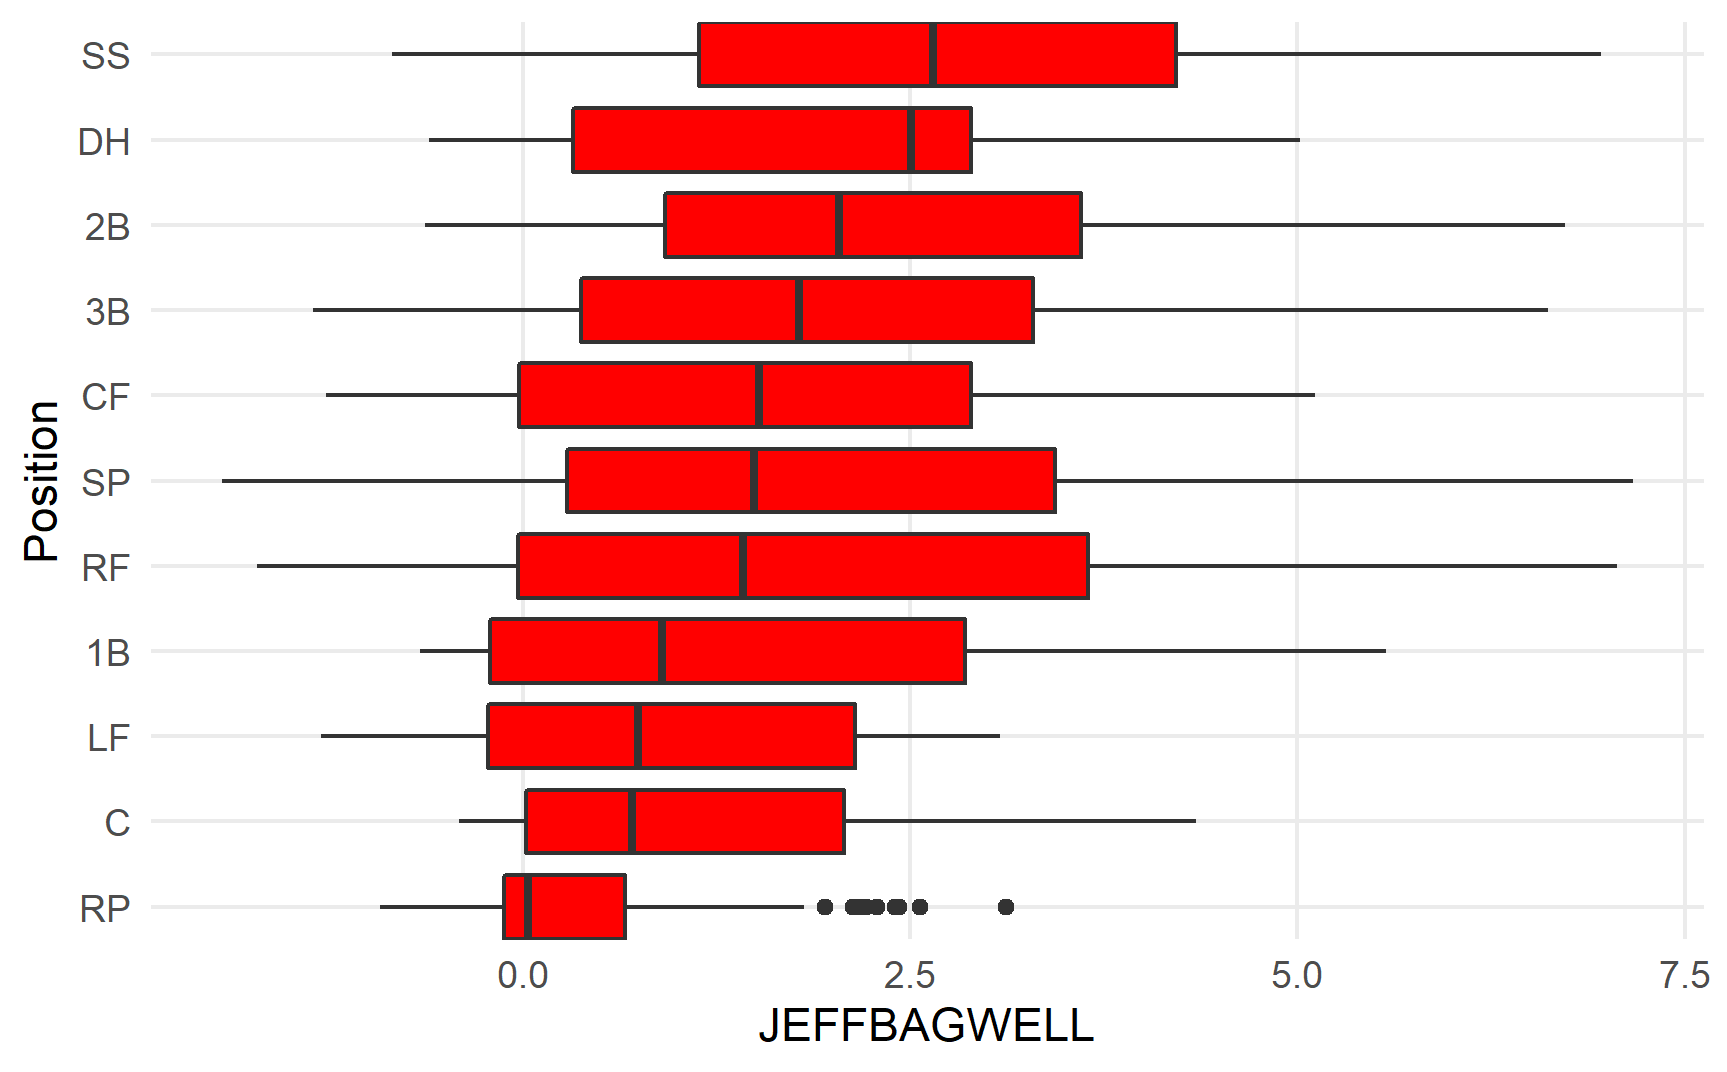
\includegraphics[width=0.7\paperwidth, scale=1.25]{war_position_boxplots.png}
\end{figure}

\section{Computational Experiment and Results}

\begin{figure}[h]
\caption{Scatterplots of a Team's Total JEFFBAGWELL vs. Total Dollars Spent for the Actual Team (Left)and Optimal Team (Right). The Red and Blue lines are constructed using LOESS.} 
\label{fig:cowplot}
\centering
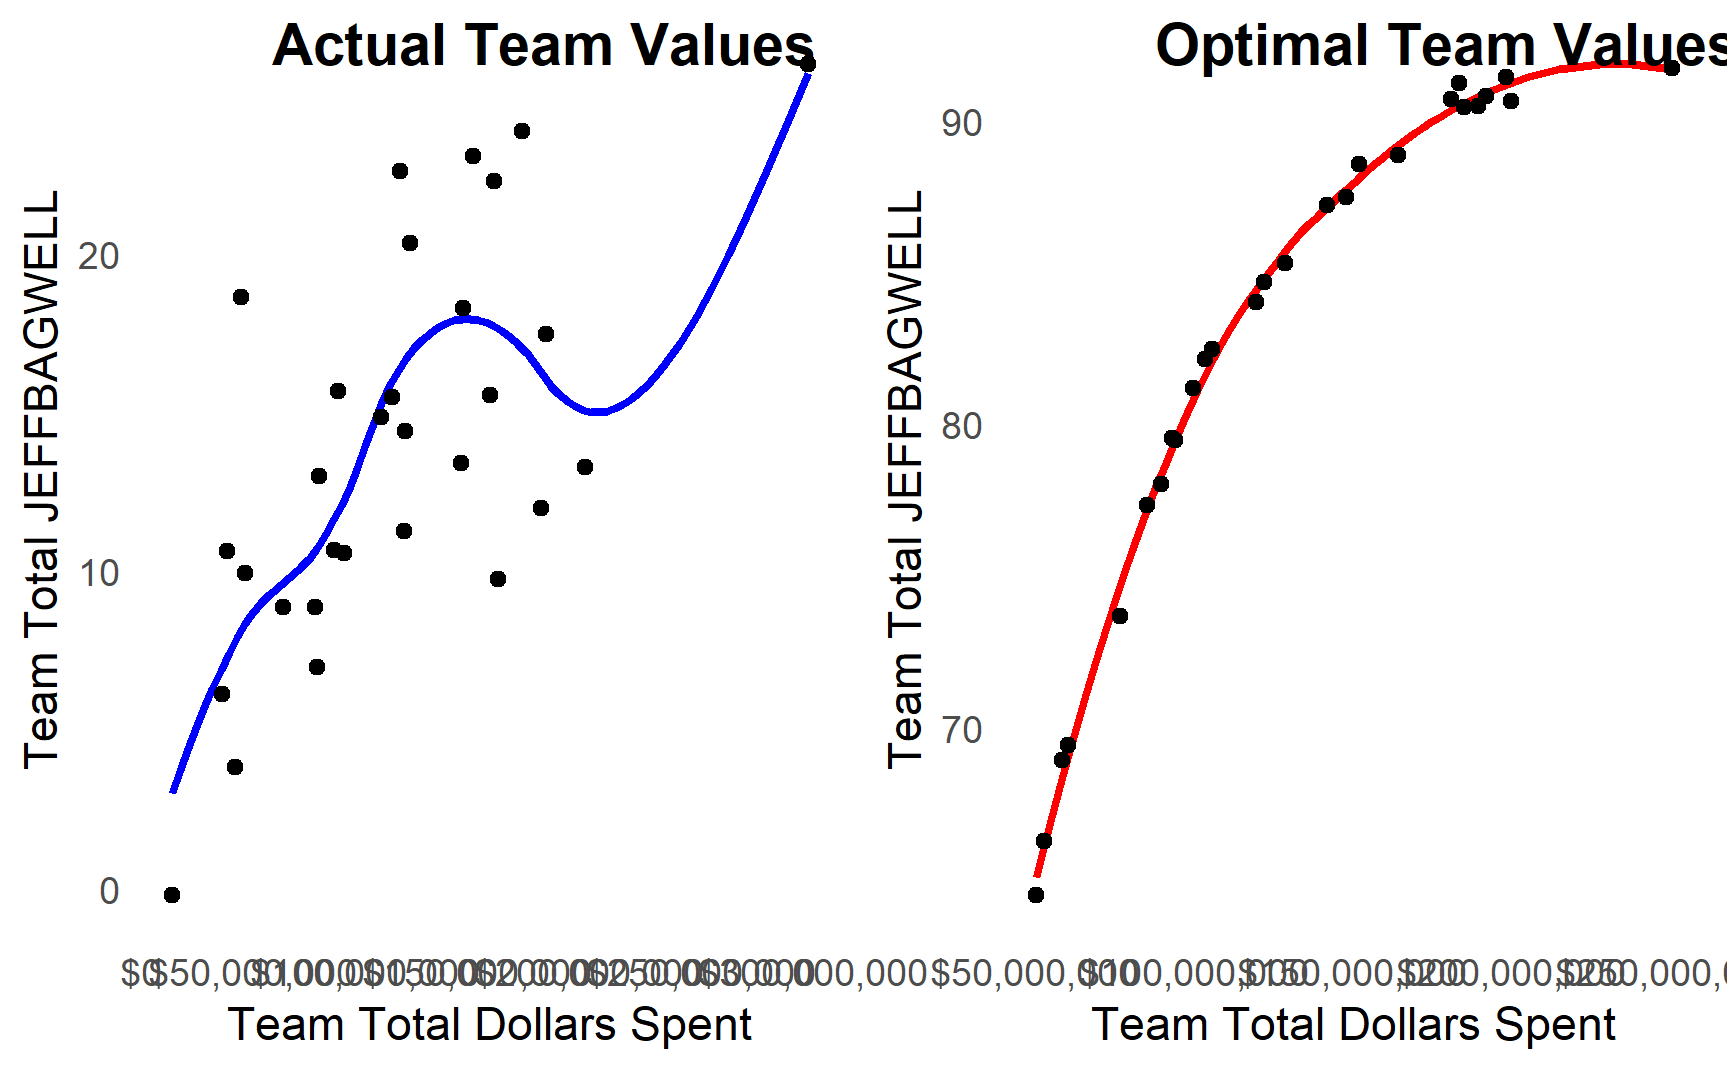
\includegraphics[width=0.7\paperwidth, scale=1.25]{bwar_salary_scatter_cowplot.png}
\end{figure}


%\begin{table}
%\caption{Five rows from the \emph{Hamilton} dataset.}
%\label{tab:example}
%\input{tables/example_raw_data.tex}
%\end{table}

\section{Discussion and Conclusions}

%\begin{figure}[h]
%    \caption{Ontology for \emph{Hamilton}. \label{fig:ontology}}
%    \centering
%    \includegraphics[width=0.7\paperwidth, scale=1.25]{ontology.png}
%\end{figure}

%\bibliography{references}
%\bibliographystyle{apalike}

\section{Appendix}

\begin{figure}[h]
\caption{Histogram of Salary for Players with Salary $> 0$}
\label{fig:salary_hist}
\centering
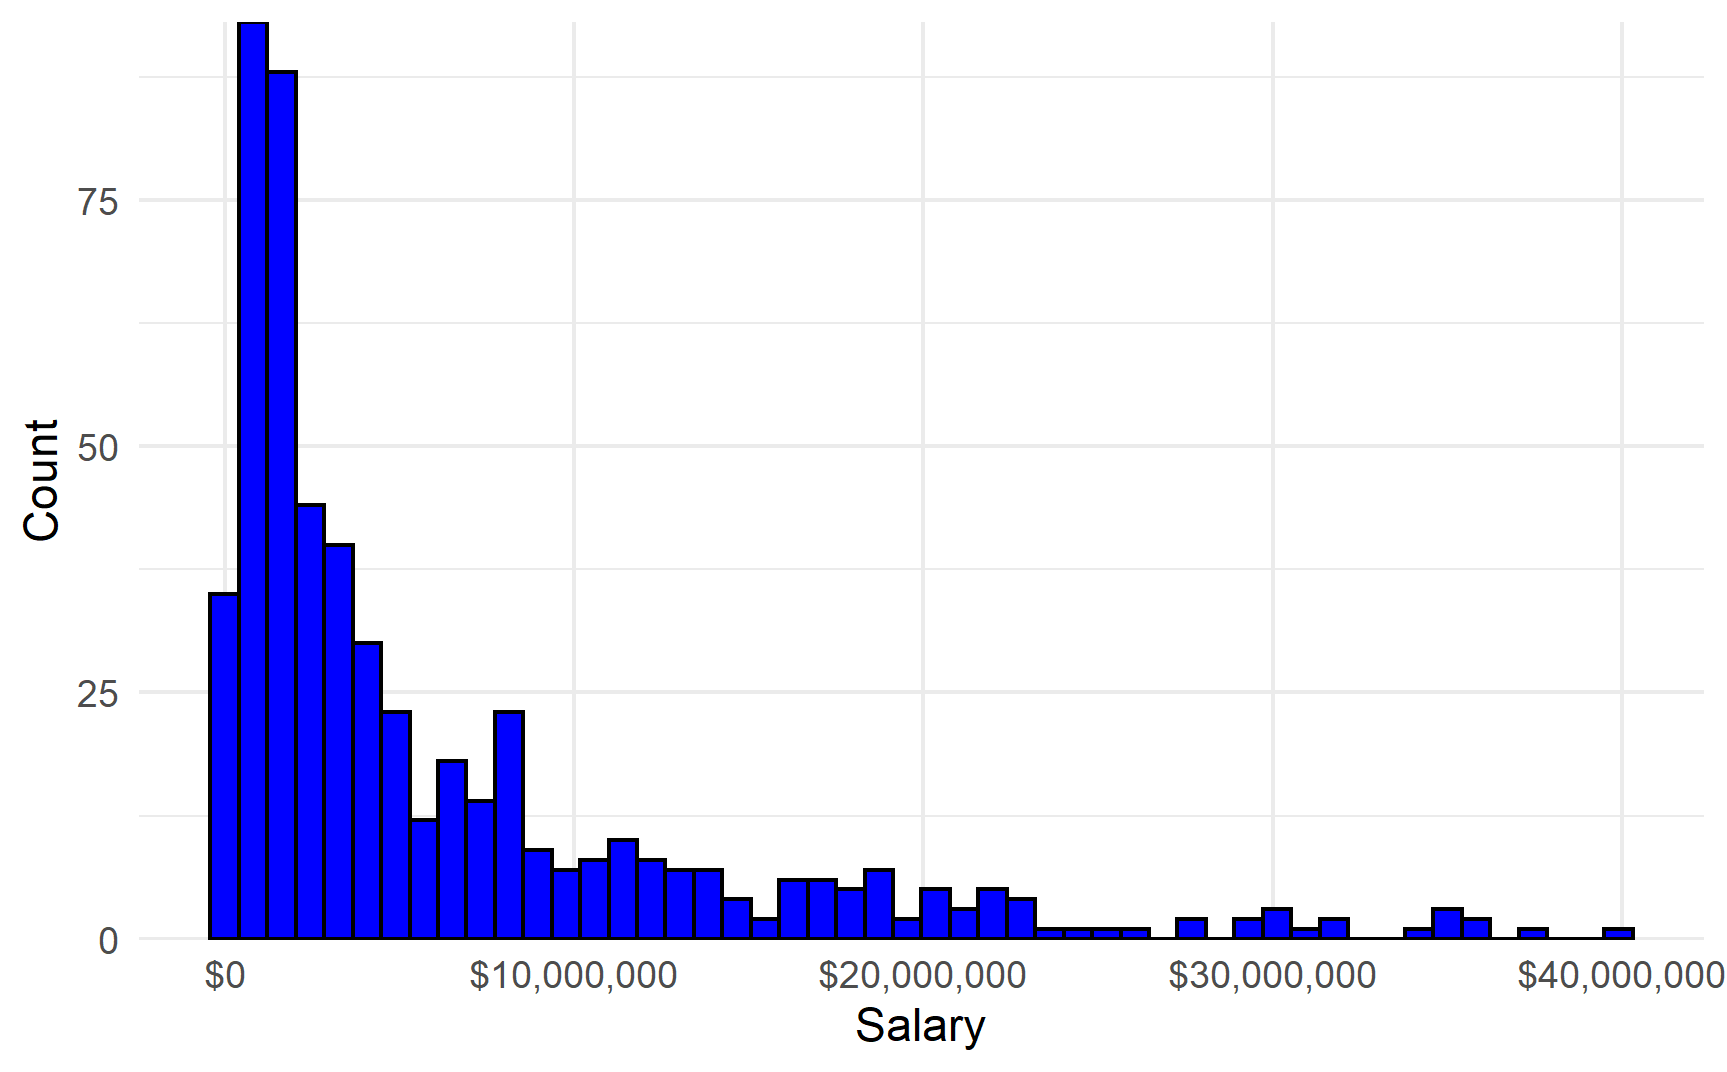
\includegraphics[width=0.7\paperwidth, scale=1.25]{salary_hist.png}
\end{figure}

\begin{figure}[h]
\caption{Histogram of JEFFBAGWELL}
\label{fig:bwar_hist}
\centering
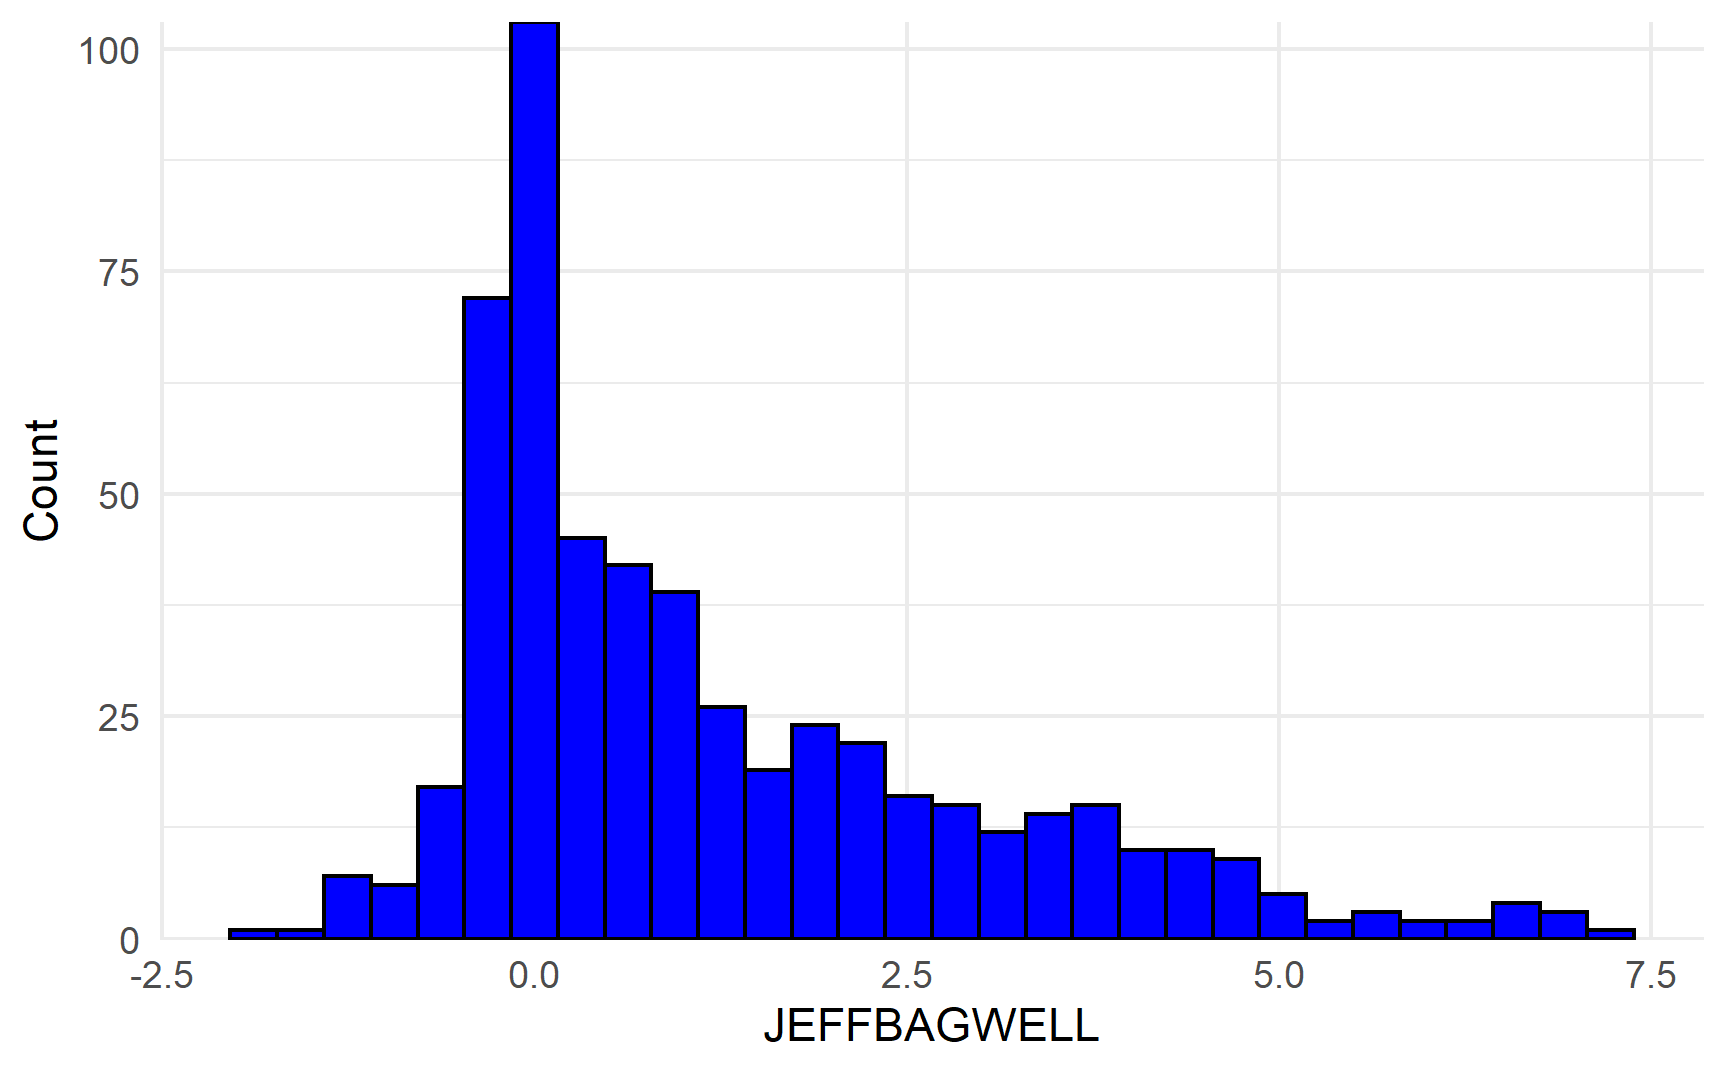
\includegraphics[width=0.7\paperwidth, scale=1.25]{war_hist.png}
\end{figure}

\begin{table}

\caption{Number of teams(max of 30) selecting player for their optimal roster}
\centering
\begin{tabular}[t]{l|r}
\hline
Player & Teams Picked\\
\hline
Darin Ruf & 30\\
\hline
Fernando Tatis Jr. & 30\\
\hline
Juan Soto & 30\\
\hline
Matt Duffy & 30\\
\hline
Matt Olson & 30\\
\hline
Shohei Ohtani & 30\\
\hline
Austin Slater & 29\\
\hline
Mike Zunino & 29\\
\hline
Jace Peterson & 28\\
\hline
Jose Ramirez & 28\\
\hline
Justin Turner & 26\\
\hline
Aaron Judge & 25\\
\hline
Carlos Correa & 25\\
\hline
Will Smith & 23\\
\hline
Andrew Albers & 22\\
\hline
Joe Ross & 22\\
\hline
Jesse Winker & 21\\
\hline
Max Fried & 21\\
\hline
Enrique Hernandez & 20\\
\hline
David Peralta & 19\\
\hline
Jacob Stallings & 18\\
\hline
Asher Wojciechowski & 17\\
\hline
German Marquez & 17\\
\hline
Brandon Lowe & 15\\
\hline
Marcus Semien & 15\\
\hline
Julio Urias & 14\\
\hline
Zack Godley & 13\\
\hline
Andy Burns & 11\\
\hline
Bryce Harper & 11\\
\hline
Scott Kazmir & 11\\
\hline
Byron Buxton & 10\\
\hline
Salvador Perez & 10\\
\hline
AJ Ramos & 8\\
\hline
Harrison Bader & 8\\
\hline
Jack Flaherty & 8\\
\hline
Joey Gallo & 7\\
\hline
AJ Pollock & 5\\
\hline
Anthony Swarzak & 5\\
\hline
Jorge Polanco & 5\\
\hline
Kyle Schwarber & 4\\
\hline
Starling Marte & 4\\
\hline
Buster Posey & 3\\
\hline
Teoscar Hernandez & 3\\
\hline
Chi Chi Gonzalez & 2\\
\hline
Jeimer Candelario & 2\\
\hline
Wade LeBlanc & 2\\
\hline
Hanser Alberto & 1\\
\hline
Jacob deGrom & 1\\
\hline
Luis Robert & 1\\
\hline
Michael A. Taylor & 1\\
\hline
\end{tabular}
\end{table}


\end{document}